%plan for this chapter


%the boring way first
- so far we have discussed constraints on reactions for invisible particles
-- remember that this is all the LHC can do by itself
- but within a single model and under certain assumptions (detector stable -> cosmologically stable), LHC results can be used to constrain properties of the parameters of DM
- and so can DD and ID, although they have the advantage that they can be sure that it's cosmologically stable DM 
- so let's put them together in this chapter, in the context of specific models, and highlight the complementarity between searches that:
-- know a lot about the interaction itself
-- can get to the origin



This extrapolation depends on the model chosen (e.g., the interaction is mediated by a Z’, or a squark, or whatever).
The collider cross-sections for invisible particle production and, separately, the cross-sections in non-collider e 

- extrapolation requires a model. lhc results are extremely model dependent but that is a feature (learn more about the model)
- complementarity: to connect particle physics to DM abundance you need dd scattering experiments.
- 


Models of particle dark matter involving SM-DM interactions necessarily link searches for DM at collider and searches in direct and direct detection experiments. Figures~\ref{fig:Complementarity} (a-c) show that, in the EFT paradigm, different search strategies are simply looking at the same process from different perspectives: DM can interact in the lab in DD experiments, it can be observed in space %galaxies is too close to snowmass formulation "indirect detection experiments that connect lab signals to dark matter in our own and other galaxies"
by ID experiments, and it can be created in the lab by colliders and observed by experiments such as ATLAS, CMS and LHCb. This complementarity of multiple experiments is necessary to elucidate the nature of dark matter in case of a discovery. Collider experiments are unable to determine whether a new phenomenon with the signatures discussed in Sec.~\ref{sec:03_ExperimentalResults} are directly connected to DM processes. % from an invisible particle or from a DM mediator. 
%Good sentence from DMF 
%One advantage of collider experiments lies in their ability to study and possibly characterize the mediator. A discovery of an anomalous E/T signature at the LHC would not uniquely imply discovery of dark matter, while at the same time e.g. discovery of an anomalous and annually-modulated signal in a direct-detection experiment would leave unanswered many questions about the nature of the interaction that could be resolved by the simultaneous discovery of a new mediator particle. Collider, direct, and indirect detection searches provide complementary ways to approach this problem [50], and it is in this spirit that much of our focus is on the mediator.

On the other hand, collider experiment can make a prediction for the signal strength of a particular model and test its consistency with relic density. This prediction can be verified in presence of a signal in DD and ID, and the connection with the galactic nature of the new phenomenon can be established. Colliders can also shed light on the physics processes that complement DM production, e.g. as in Fig.~\ref{fig:Complementarity} (d) colliders can discover the new particle mediating the interaction and measure its coupling to SM particles other than quarks and gluons, or they can observe other cascade decays that produce the DM particle in case of SUSY models. For this reason, it is important to have a broad LHC search program that includes different experimental targets, both generic and model-specific.  %would be nice to give some literature here but no space

\begin{marginnote}[]
\entry{The LHC Dark Matter Working Group}{did this} 
\end{marginnote}. 

JUNK: Axial vector are the most widely used LHC benchmarks as DD rates are suppressed. 

JUNK: Since the pseudoscalar model has been favoured for the interpretation of the DAMA and galactic center excess~\cite{Arina:2014yna,Agrawal:2014una} and collider searches are favored when comparing to DD~\cite{Banerjee:2017wxi}, LHC searches have privileged this choice and considered the associated scalar boson as decoupled at higher energies. 


%Note on this figure: it's on wikimedia before i submitted the nature physics because I planned to reuse it here and told nature physics i wanted it cited but nature physics being the predatory shit paper that it is ignored all my request of creative commons (but they redid it with thinner lines). maybe we reword the caption?
\begin{figure}[!htpb]
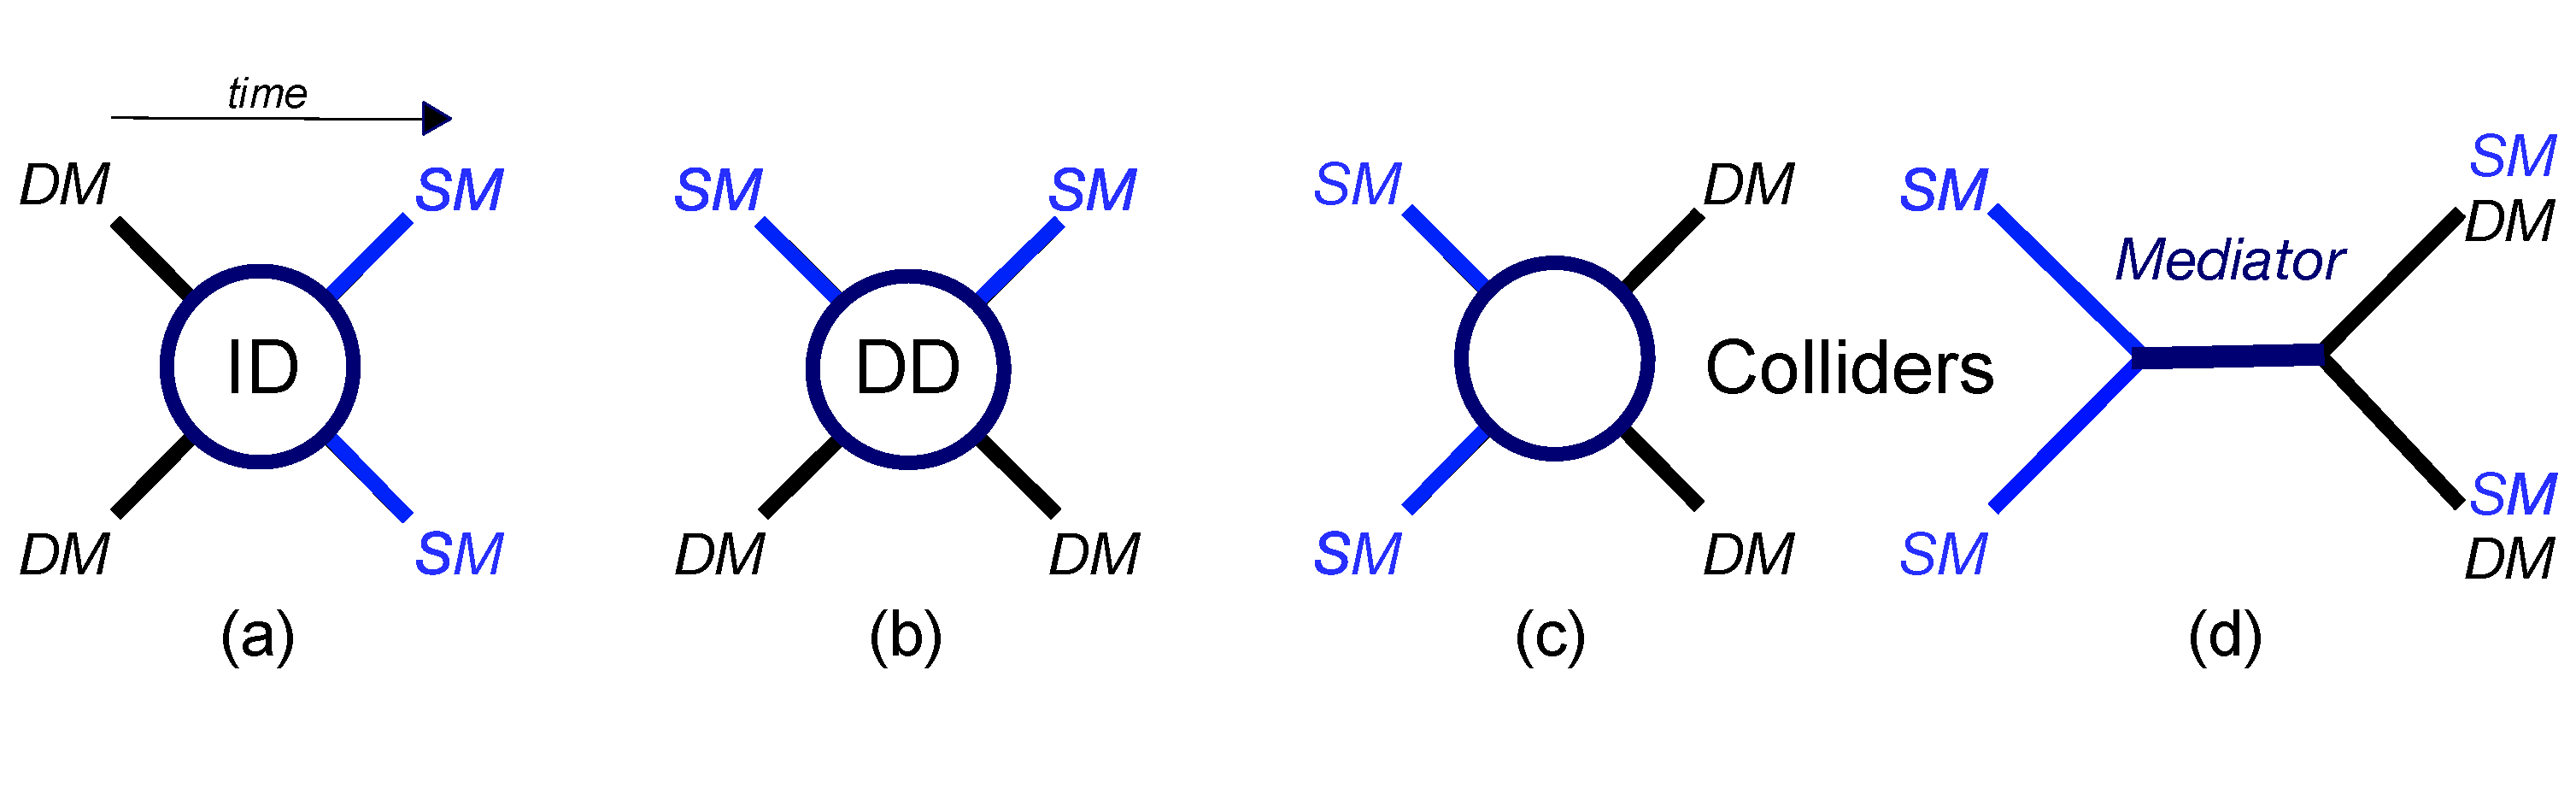
\includegraphics[width=\textwidth]{figures/EFTSimplifiedModels}
\caption{Schematic illustration of Dark Matter interactions and their corresponding experimental detection techniques, with time flowing from left to right. Fig. (a) shows DM annihilation to Standard Model particles, as sought by Indirect Detection (ID) experiments. Fig. (b) shows DM -> SM particle scattering, targeted by Direct Detection (DD) experiments. Fig. (c) shows the production of DM particles from the annihilation of SM particles at colliders. Fig. (d) shows again the pair production of DM at colliders as in (c), but in this case the interaction occurs through a mediator particle between DM and SM particles. From~\cite{monoXfig}, inspired by ~\cite{Bauer:2013ihz}.}
\label{fig:Complementarity}
\end{figure}

It is also worth mentioning that, even though comparisons between collider, DD and ID are becoming the standard for these communities,
the comparison with LHC, DD and ID results with results from astrophysics beyond the relic density is a growing field. 
This is particularly important since all the observational evidence of DM that we have is gravitational,
so DM properties such as mass and density in our and other galaxies
can be inferred from galaxy simulations or deviations in astrophysical observables, 
and signatures of DM self-interactions in rotation galaxies or cluster collisions can complement and verify any DD 
observations. Even though we do not cover this topic in detail in this review we refer to~\cite{Buckley:2017ijx}. 

\subsection{Comparing LHC constraints from visible and invisible searches with non-collider results}

The comparison of results from complementary experiments needs a mechanism to relate the processes
that will produce a signal in each type of detectors. This ultimately means that any comparison between LHC, DD and ID
needs a fully specified theoretical benchmark to be predictive and consistent. Since there are a large possible number of options to choose from, it is always important to keep in mind that such comparisons are model-dependent and the choice of benchmark can have severe implications for the conclusions drawn. 

%%LHC -> DD/ID

%EFT
Tevatron and Run-1 LHC searches mainly used EFTs as the common theoretical ground to compare their constraints on DM across experiments, or full models such as SUSY. EFTs are a good and flexible benchmark model to represent DM interactions in DD and ID experiment, since the momentum transfer of the collision is sufficiently low not to resolve the theory beyond the scale of the interaction and certainly below the electroweak scale. As discussed in Sec.~\ref{sub:EFT}, this is not always the case for high-energy collider experiments. The difference in interaction scales also requires that any operator in the model is evolved from the scale of the LHC collisions to the nuclear scale of DD through renormalization group expansion (RGE)~\cite{DEramo:2014nmf} for full consistency of the results. %is it clear enough that this has to be done for simplified models too? 
An example of a comparison plot between collider and DD results using EFT operators in the WIMP-nucleon cross-section vs WIMP mass plane\footnote{The formulas to translate LHC limits to this plane can be found in Ref.~\cite{Goodman:2010ku}}, without evolving the operators using RGE but showing the effects of the truncation of the events where the EFT is invalid, is shown for the LHC Run-1 results in Fig.~\ref{fig:SIATLASEFT}. %There isn't enough space to describe the results of the truncation in detail
What can be inferred from the plot is that within this class of models and spin assumption %We could have a footnote on SD and SI but no room in text?
the ideal region for the discovery of DM is that where WIMPs have masses above 10 GeV, as both collider and DD experiments are sensitive and could verify each other's claims. Next-generation DD experiments are expected to lower the minimum sensitivity thresholds in the next decade, see e.g.~\cite{Agnese:2016cpb}. 

\begin{figure}[!htpb]
%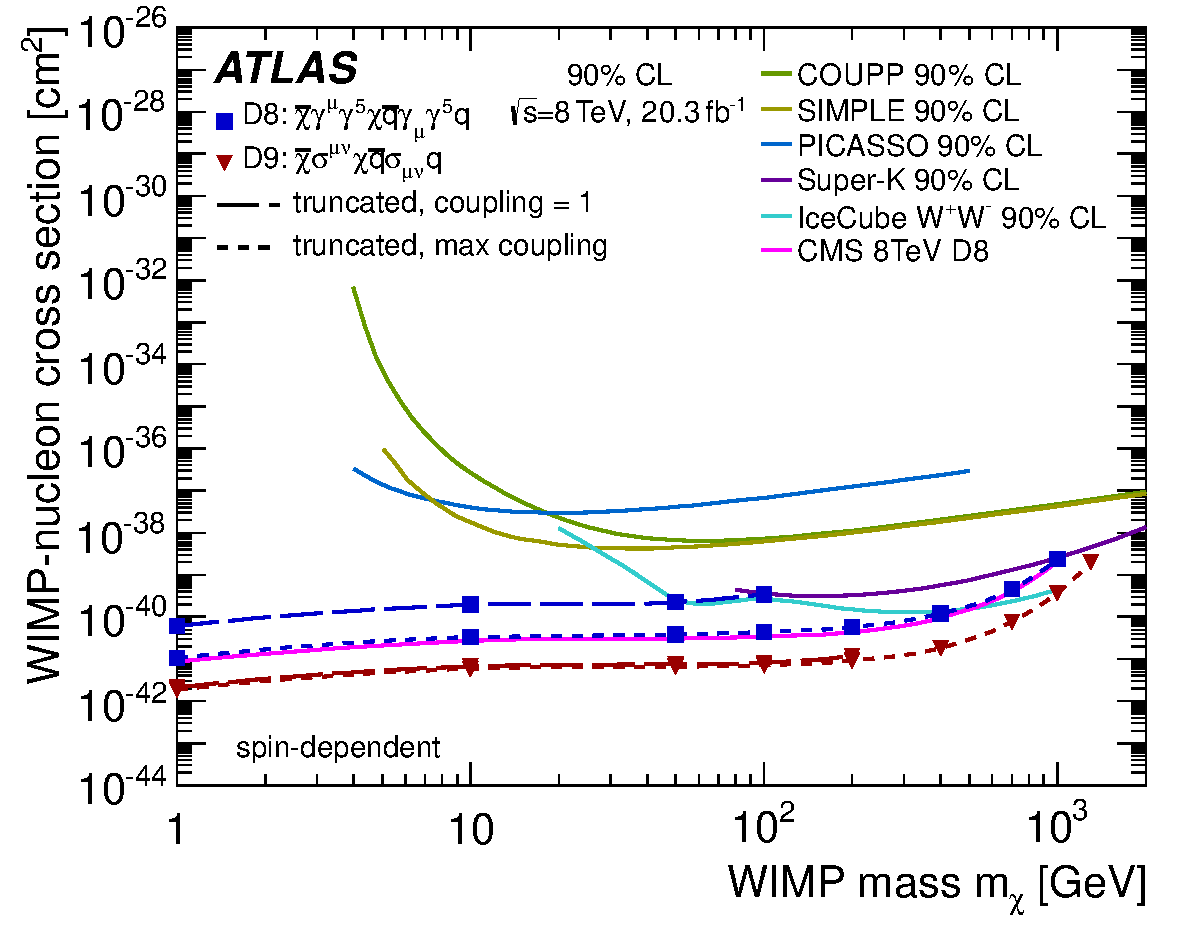
\includegraphics[width=0.35\textwidth]{figures/Monojet8TeV_EFT_SD}
%Can't have both so choose less controversial
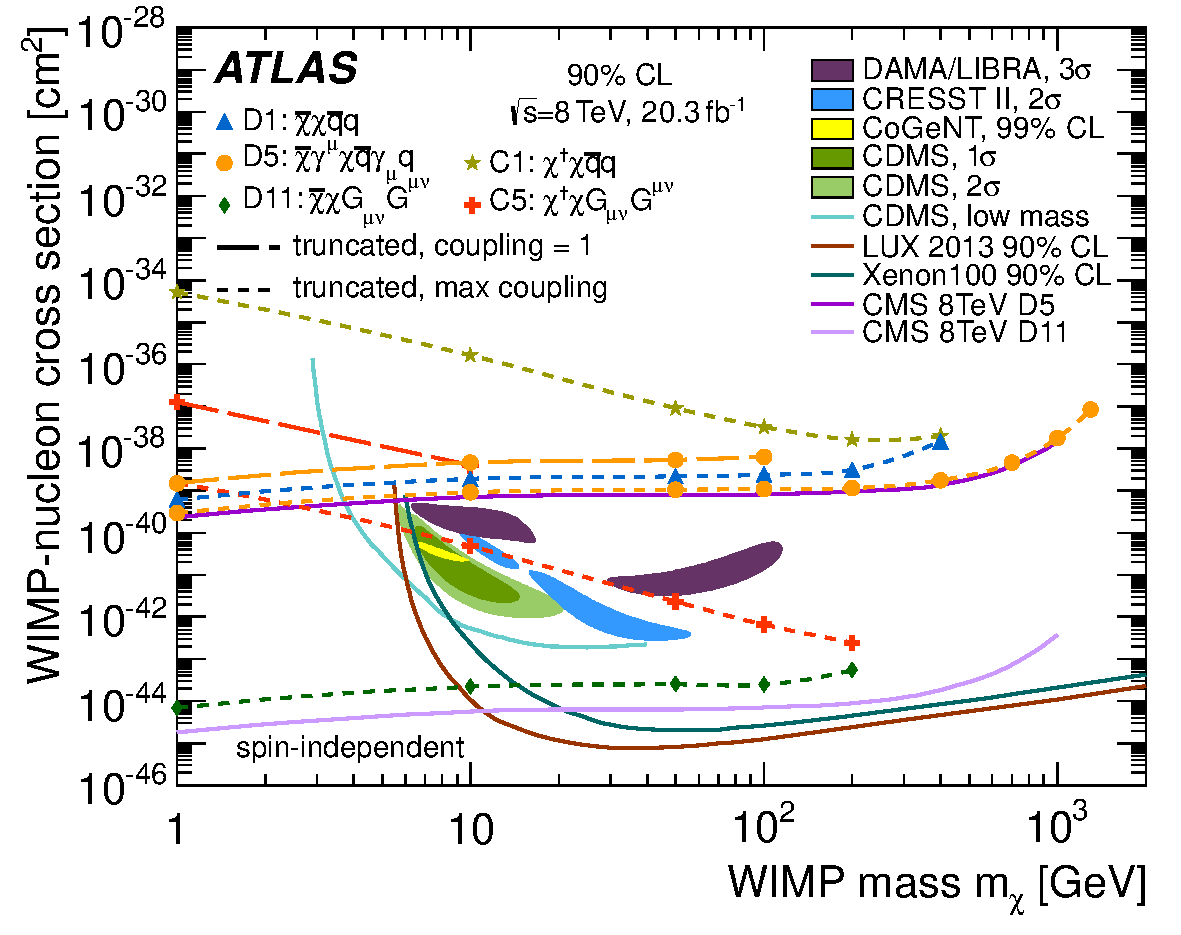
\includegraphics[width=0.9\textwidth]{figures/Monojet8TeV_EFT_SI}
\caption{Inferred 90\% CL limits on (left) the spin-independent and (right) spin-dependent WIMP--nucleon scattering cross section as a function of DM mass m? for different operators. Results from direct-detection experiments for the spin-independent and spin-dependent cross section, and the CMS (untruncated) results are shown for comparison. From~\cite{monoXfig}.}
\label{fig:SIATLASEFT}
\end{figure}

%Simp

\begin{figure}[!htpb]
%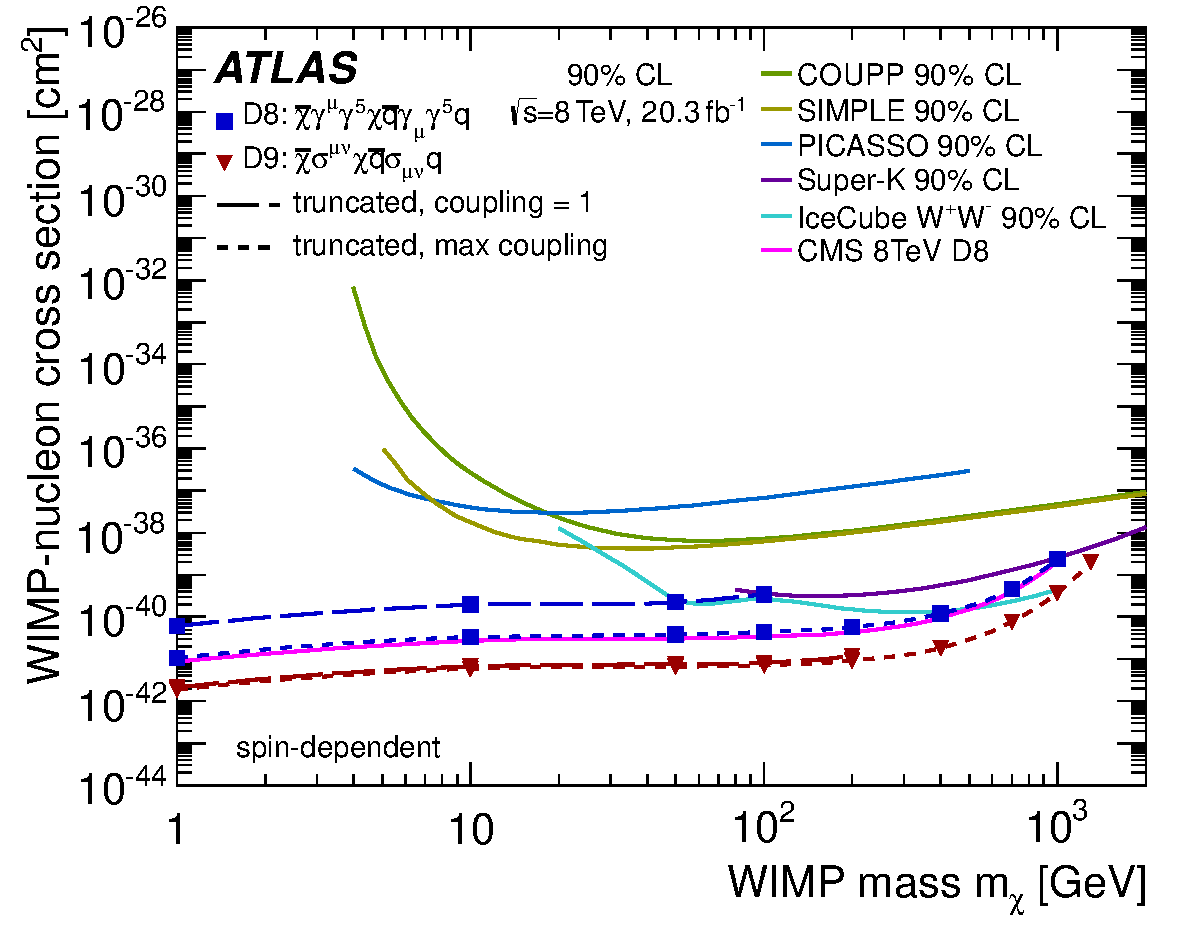
\includegraphics[width=0.35\textwidth]{figures/Monojet8TeV_EFT_SD}
%Can't have both so choose less controversial
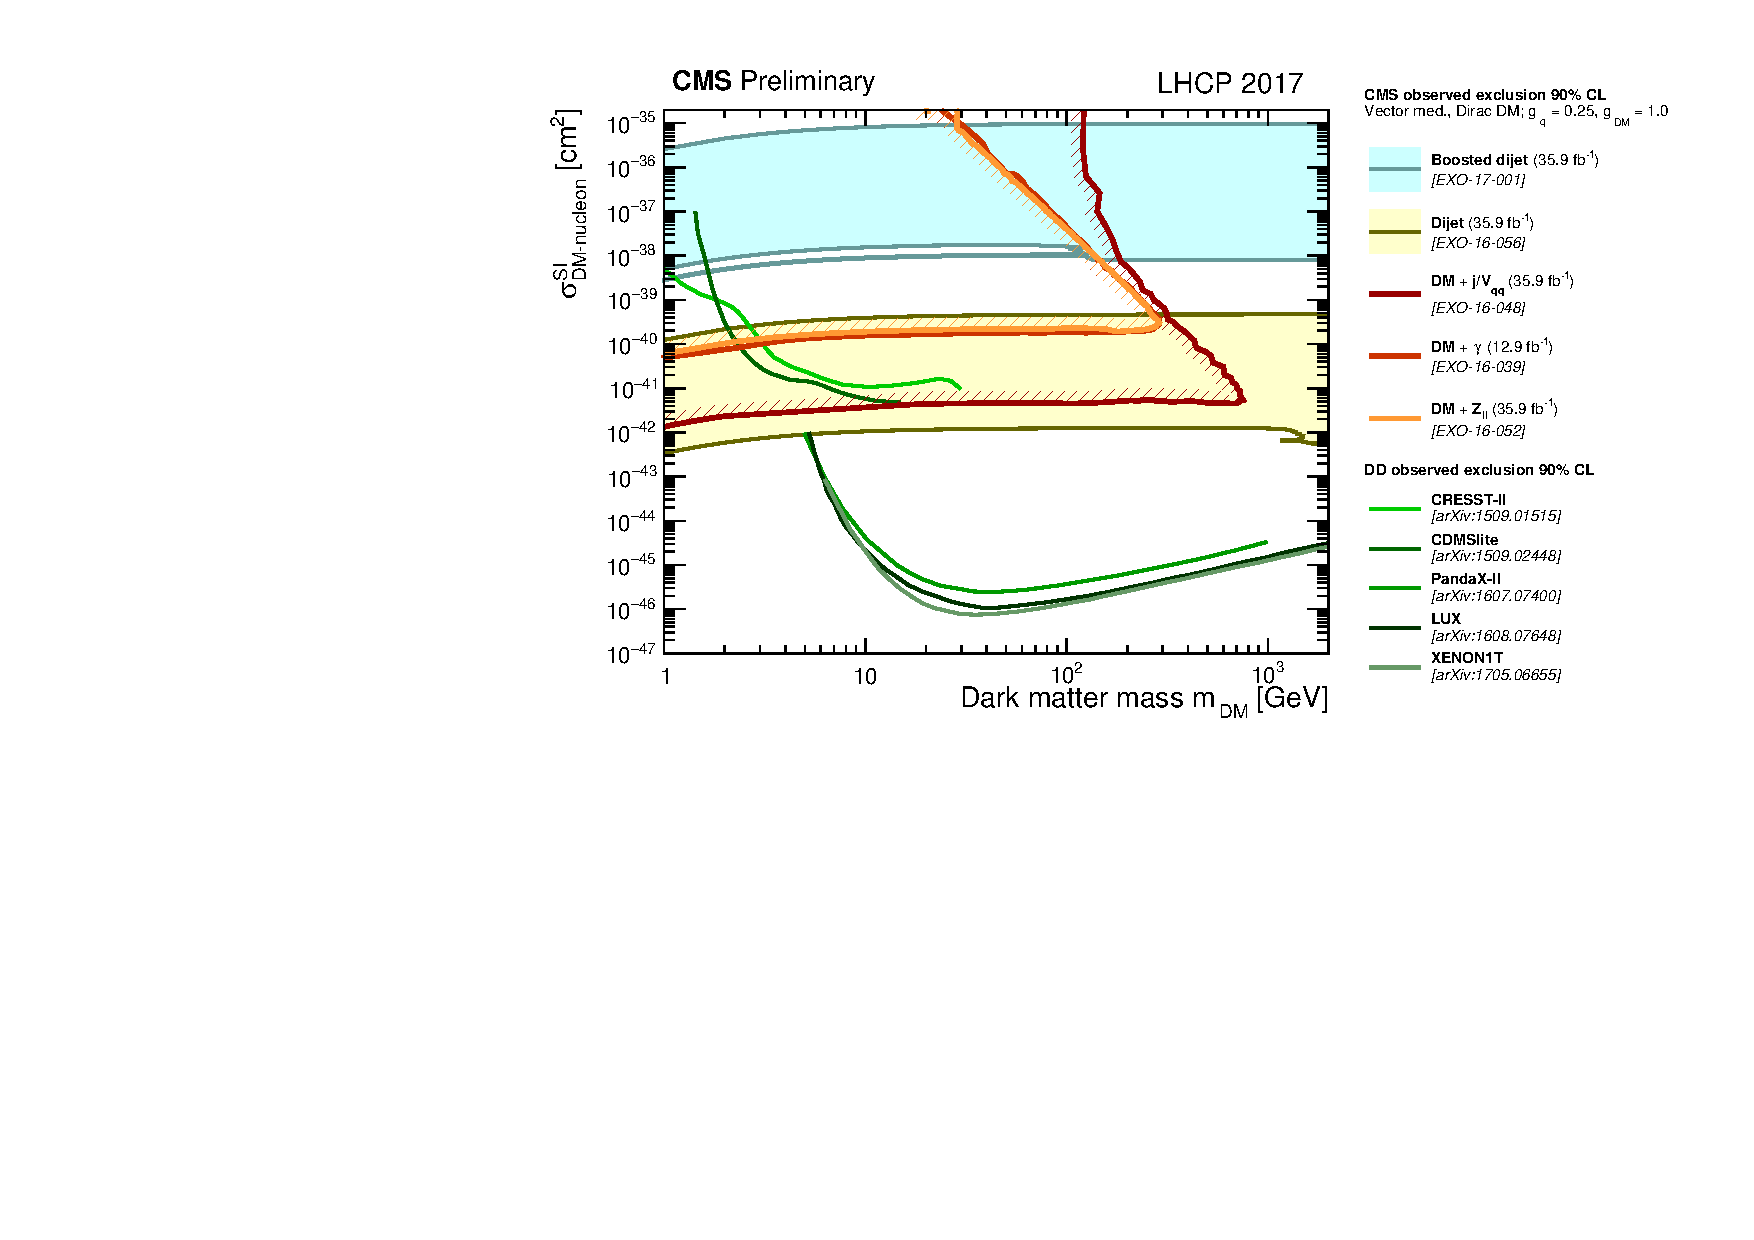
\includegraphics[width=0.9\textwidth]{figures/SI_CMSDD_Summary}
\caption{The 90\% CL CMS constraints in the \mdm-spin-independent DM-nucleon plane, for a vector mediator, Dirac DM and couplings gq = 0.25 and gDM = 1.0, compared with DD experiments. From~\cite{CMSSummary}.}
%We can update if something else comes out
\label{fig:SICMS}
\end{figure}
%Q: use SD? it will piss off more people but maybe we could make that point as well
%We could cite PDG review on spin-dependent vs spin-independent

With the adoption of simplified models of DM by LHC searches in Run-2~\cite{Abercrombie:2015wmb}, the
constraints and caveats of the comparisons between DD and ID have been made clearer, even though the comparisons themselves have become more model-specific and so far privileged vector and axial vector $s-$channel models with fixed coupling values. ATLAS and CMS follow a series of recommendations and well-defined procedure by the Dark Matter Working Group~\cite{Boveia:2016mrp}. LHC experimentalists and theorists have chosen to translate the collider results on visible mediator and invisible DM searches from the \mdm, \mmed plane to the DD and ID planes, so that all information on the results that are reinterpreted are available and all assumptions can be clearly spelled out. An example of such a comparison including the most recent LHC and DD results is shown in Fig.~\ref{fig:SICMSEFT}. In this kind of comparisons, it should be noted that the colliders limits do not include any constraint on the relic density, and that absolute exclusion of the different collider searches as well as their relative importance depend strongly on the benchmark scenario and its coupling. We also note that neither this procedure nor the benchmark models used are explicitly accounting for effects that may be important for mediators with masses below 100 GeV, such as interference and mixing with the X boson, quarkonia resonances and unitarity violation. 
%Could cite this for more consistent w/completion and ID: Jacques:2016dqz, but not sure what it adds, I prefer to talk about Linda's result
For reinterpretation of LHC results and their comparisons to DD and ID for scalar and pseudoscalar mediators, also in the context of 2HDM, see e.g.~\cite{Athron:2017kgt,Banerjee:2017wxi,Ipek:2014gua,Bell:2016ekl}.
%Proposals exist so that the plots should be truncated for cross-sections corresponding to a minimum mass.  
%Q: mention discussion from Landsberg? Would be nice. 
%https://indico.cern.ch/event/563066/contributions/2306614/attachments/1340042/2017991/DMWG-09-20-16.pdf
%Mention how low can one go in mdm - AB knows better here? 
%%DD/ID -> LHC
The comparison of collider and ID results using simplified model benchmarks has received new attention since the publication of~\cite{Boveia:2016mrp}. In traditional comparisons, only one DM annihilation state at a time has been used for the comparison of collider and ID results (e.g. $b\bar{b}$, see for example~\cite{Agrawal:2014una}). The work in~\cite{Carpenter:2016thc} considers multiple final state fermions and interprets ID and LHC results in simplified models with $s-$ and $t-$channel mediators. 

Recently, LHC results have also started to be utilized by DD collaboration for constraints of simplified models of DM, see e.g.\cite{PhysRevLett.118.251301,Balazs:2017hxh}. IceCube and other experiments have used constraints from a MSSM scan, see e.g.~\cite{Aartsen:2016zhm}. The pMSSM is also a good framework to highlight the complementarity of LHC, direct and indirect detection experiments, as shown in e.g. Ref,~\cite{Cahill-Rowley:2014twa}.  %CD: maybe add some quantitative results?

%Would be nice to have a figure but probably too complicated to get as it's published

%Mention Gambit? I would rather describe it in the "SUSY fits" part

%We aren't talking about uncertainties on DD and ID, maybe we should or at least we should cite?
%https://arxiv.org/abs/1409.5446

All experimental results, be it from DD, ID or collider, are affected by experimental and theoretical uncertainties.
%"We advocate that": not sure i want to put that in
A further step towards a more informative comparison between these results is to convey 
an idea of the impact of those uncertainties in the plots. 
The main uncertainties for LHC searches have been outlined in Sec.~\ref{03_ExperimentalResults},
and they are traditionally displayed as one-sigma bands around the LHC constraints. 
Additional uncertainties in the procedure that translate collider results in the DD and ID planes
stem from the matrix elements of the nuclei, but this is an uncertainty that
affects DD as well. %Could make this clearer and cite? 
The situation is less straightforward when comparing collider results to measurements subject to astrophysical
uncertainties (for a summary of DD and ID uncertainties, see~\cite{Feldstein:2014ufa,d300ef23986a49099715e661295a4d72}
and references therein) as those are difficult to estimate and can have a large impact that affects 
different kinds of experiments differently. 
The experimental and theoretical communities have not yet agreed on a common presentation of experimental uncertainties, 
but we expect the discussion will continue in the future. 

\subsection{Comparing LHC constraints from visible and invisible searches with the DM relic density}

%need to match this with the stuff in the introduction and make sure it does not repeat
The observed abundance of DM in the universe today, derived from fits of the Cosmic Microwave Background
measured with the Planck satellite~\cite{Ade:2015xua}, is one
of the few %the only? 
available quantitative DM observations. 
As shown in Fig.~\ref{fig:sensitivityComparison} LHC experiments overlay a line corresponding to 
a dark matter density of $\omega_c = 0.12 h^2$ according to the standard thermal history as calculated
from programs such as MadDM and MicrOMEGas~\cite{Backovic:2015cra,Barducci:2016pcb}, to 
illustrate where a given simplified model is sufficient to explain the observed DM abundance. 

Conclusions on whether a model is ruled out by information on relic density alone cannot be drawn for simplified models, 
as there may be additional physics processes beyond those included in the simplified model that influence the DM abundance.
Moreover, the assumption of a standard thermal history where the current DM density is achieved via freeze-out  
%does the reader know what a standard thermal history is?
%how do we treat the assumption of LambdaCDM? way too big a discussion to start here
is only one of the possibilities~\cite{Bernal:2017kxu}. 
Nevertheless, the relic density remains a useful guiding principle for DM searches if these assumptions are correct~\cite{Busoni:2014gta,Catena:2017xqq}. 

%Confronting the entire set of collider results with the relic density using a full model requires a 
%careful framework that is able to test model points against data. A variety of tools are available for this purpose,
%notably Mastercode~/cite{MC} and Gambit~/cite{G}. [Do we want to describe? Sentence is empty this way but we have no more space]. 

%DMWG 
%Relic density calculations can be overlaid on the mass-mass plot to indicate where the particles and interactions of a specific simplified model are by themselves su cient for explaining the observed DM abundance. For the simplified models recommended by the ATLAS/CMS DM Forum, this curve corresponds to the parameters for which the observed relic abundance is compatible with a single species of DM Dirac fermion and a single mediator that couples to all SM quarks with equal strength. One should not conclude that a simplified model is ruled out for values of model parameters that are inconsistent with the relic density overlay. Rather, one should conclude that additional physics beyond the simplified model was relevant for determining the DM abundance in the early Universe.



%%%%%THIS IS ALL STUFF FROM CHAPTER 3

\subsection{Stuff from chapter 3}

\subsubsection{monoZ}
%MonoZ


The LEP precision measurements~\footnote{Bounds on Z to invisible decays obtained from LHC searches are not yet competitive~\cite{deSimone:2014pda}.}, as well as direct detection experiments, rule out the majority of the Z-mediated invisible particles scenarios~\cite{Arcadi:2014lta,Escudero:2016gzx}. The LEP invisible width is well below the width one would expect if vector and axial vector models of invisible particles were realized, for all couplings satisfying the relic density with a invisible particles mass below 25 GeV. Direct detection experiments such as Xenon1T~\cite{Aprile:2017iyp} 
%CD: take figure 2 of Escudero:2016gzx and compare with the results of Aprile:2017iyp
rule out most of the other simplified model scenarios compatible with freeze-out relic density up to multi-TeV invisible particles masses. 
%invisible particles mass above 6 TeV for the vector couplings, while for axial the plot is truncated. 

%%Text from before

The invisible decays of the Z and Higgs boson are the main direct targets of searches for SM-boson-mediated interactions between SM and invisible particles particles, if the invisible particles particle is lighter than half the mass of the boson. Above this region, Direct Detection experiments are generally more sensitive than collider experiments. 


If the invisible particles mass is below half the mass of the Z, the Z can decay into invisible particles leading to strong constraints by LEP. Direct detection experiments constrain the rest of the parameter space 
where the relic density is satisfied. 
constrained by LEP and direct detection experiments (see e.g. Refs.~\cite{Arcadi:2014lta,Escudero:2016gzx}).

In $SU(2)_L \times U(1)$ extensions of the SM, the axial and vector couplings of the Z boson to invisible particles are generally required to be of the same order. If no other couplings are present, this model is not $SU(2) \times U(1)$ invariant, unless couplings to the invisible particles to the Higgs boson are added as well~\cite{Kahlhoefer:2015bea}. 
%The couplings between the Z and the invisible particles can be vector, axial or mixed. 
In the minimal case where the couplings do not depend on the Lorentz structure of the interaction, 
%what I want to say: In general they are excluded in their minimal version because of their strong vectorial coupling necessary to respect relic abundance bounds.
large couplings are required for this model to satisfy the relic density. 
In the case of equal vector and axial couplings, this model is heavily 

This model can still be viable wherever no relations between the vector and axial couplings are present. A review of Z portal models with different couplings can be found in Ref.~\cite{Arcadi:2014lta}. 
%Does one require a certain kind of couplings for symmetries? 
%Arcadi says: 
%In all these extensions, the axial coupling Aχ (see eq.(1)) of the Z boson to the invisible particles is naturally of the order of magnitude of its vectorial coupling Vχ. The deep reason is that in a framework of SU(2)L × U(1) breaking the original SU(2)L condition (Vχ = Aχ) is only mildly modified by the dynamic of the breaking. 
%Maybe link this to the choices for the Z' model later on? 

%%End text from before

\subsubection{H portal}

%What does it mean for Higgs portal models: DD is always better
In the case of light fermion invisible particles with scalar couplings to the Higgs, direct detection experiment rule out most of the parameter space where the model can provide the measured relic density~\cite{Escudero:2016gzx,Djouadi:2011aa}. Due to the suppression of the cross-section for DD in the pseudoscalar case, the model is still not constrained around a small region for invisible particles masses corresponding to half the Higgs mass and above. %CD: maybe we have to say why this is the case - essentially rates are too small, see paper by Plehn. 

\subsubsection{Monojet}

%V/AV come from CMS search, ATLAS is less sensitive as it's 1.55 TeV
Vector and axial vector mediators are excluded by LHC searches at values of \minvisible particles up to 700 and 400 GeV respectively with \mmed up to 1.8 TeV. This choice of model and couplings produces a relic density that is lower than the Planck measurement and it is still unconstrained by LHC searches for \minvisible particles$>$0.3 TeV at \minvisible particles$=$1.8 TeV for the vector mediator, and for 0.65$<$\minvisible particles$<$0.75 TeV at \minvisible particles=1.8 TeV for the axial vector mediator\footnote{Here and in the following, we quote observed limits at 95\% C.L. and refer to the bibliography for expected limits and 90\% C.L. limits.}. 
